\documentclass[lang=cn,10pt,device=pad]{elegantbook}
%titlestyle=display
%toc=twocol
\title{《拓扑学》学习笔记}
\subtitle{基于庄晓波老师的教学视频and一些不知道从哪里来的idea}
%($\subset my$的)
\setCJKmainfont[ItalicFont=FandolKai-Regular,BoldFont=STSongti-SC-Black]{STSong} 
\setCJKsansfont{FandolHei-Regular}
\setCJKmonofont{FandolFang-Regular}
\setCJKfamilyfont{kaiti}{FandolKai-Regular}
\setCJKfamilyfont{cusong}{STSongti-SC-Black}
\setCJKfamilyfont{fang}{FandolFang-Regular}
\newcommand{\kaiti}{\CJKfamily{kaiti}}%\
\newcommand{\cusong}{\CJKfamily{cusong}}%\
\newcommand{\fang}{\CJKfamily{fang}}%
\usepackage{calligra}

\author{张博涵}
\institute{张博涵}
\date{起著重庄赤奋若}
\version{\today}
%\version{1.0}
\bioinfo{Github地址}{\href{www.github.com/BHanZhang}{www.github.com/BHanZhang}}

\extrainfo{摄于2022年07月28日~河南省~洛阳市~~{\calligra with}~{\calligra my}~{\calligra my}}

\setcounter{tocdepth}{3}

%\logo{logo-blue.png}
\cover{cover.jpg}

% 本文档命令
\definecolor{mygrn}{RGB}{21,153,65}
\definecolor{myor}{RGB}{252,113,21}
\definecolor{myblu}{RGB}{46,90,168}
\usepackage{array}
\newcommand{\ccr}[1]{\makecell{{\color{#1}\rule{1cm}{1cm}}}}
\newcommand{\tl}[1]{\textcolor{myor}{#1}}
\newcommand{\gn}[1]{~\textcolor{mygrn}{\cusong{#1}}~}
\newcommand{\lei}[1]{~\textcolor{myblu}{\cusong{#1}}~}
\newcommand{\tp}{\mathscr{F}}
\newcommand{\tpj}{\mathcal{B}}
\newcommand{\mj}[1]{\mathscr{P} (#1) }
\newcommand{\st}{~s.t.~}
\newcommand{\dabing}{\displaystyle\bigcup}
\newcommand{\dajiao}{\displaystyle\bigcap}
\newcommand{\dkh}[1]{\{#1\}}
\newcommand{\xkh}[1]{\left(#1\right)}
\newcommand{\chadiao}{\backslash}
\newcommand{\ranhou}{\Longrightarrow}
% 修改标题页的橙色带
\definecolor{customcolor}{RGB}{249,125,28}
\colorlet{coverlinecolor}{customcolor}

% 图片并排
\usepackage{paracol}
\columnratio{0.5}           % 栏宽比例
%\setlength{\columnsep}{0em} 
%\setlength{\parskip}{.5ex plus 1pt}
\normalcolseprulecolor[black]
\setlength{\columnseprule}{0.4pt}
\newcommand{\zhu}[1]{\end{paracol}
\begin{paracol}{2}
\switchcolumn
#1
\vfill
\switchcolumn
}

\begin{document}

\maketitle
\frontmatter

\tableofcontents

\mainmatter
%第一章
\chapter{拓扑空间}
\section{拓扑空间,开集}
\begin{definition}[拓扑空间,开集]\label{c1-d1}
	设$X$为一个集合$\mathscr{F}\in \mathscr{P}(X)$(把$\mathscr{F}$中的元素称为$X$中的\gn{开集}),满足:
	\begin{enumerate}
		\item $\emptyset , X \in \mathscr{F}$
		\item $U , V$是开集,那么$U\cap V$是开集
		\item $U_{\alpha} , \alpha\in I $是开集,$\dabing_{\alpha\in I}U_{\alpha}$是开集。
	\end{enumerate}
	则称$\mathscr{F}$为$X$上的一个\gn{拓扑},$(X,\tp)$为一个\gn{拓扑空间}。
\end{definition}

\begin{note}
	有时候这样写:“设$X$为拓扑空间”,这就意味着“$X$为一个集合,且规定了$X$上的一个拓扑(指定了那些子集为开集)”。
\end{note}


\begin{note}
	这里第二点可以更换为“有限个开集的交仍为开集”,这样的定义也与我们熟知的开集的性质相一致。
\end{note}
\begin{example}[欧氏拓扑]
	对于$n$维欧氏空间$\mathbb{R}^{n}$,$\tp  = \{\mathbb{R}^{n} \text{在通常意义下的开集} , \emptyset\}$构成一个拓扑空间。
\end{example}
\begin{proof}
	验证其为拓扑空间,就是要验证三条:
	
	\begin{enumerate}
		\item 第一条显然成立 : $\emptyset , \mathbb{R}^{n} \in \mathscr{F}$;
		\item 设$U,V$为$\mathbb{R}^{n}$中开集,要证$U\cap V$为开集。任取$x_{0}\in U\cap V$,就有:
		\begin{enumerate}
			\item $x_{0}\in U$ ,有$\exists \delta_{1} , \st   x_{0}\in B(x_{0},\delta_{1})\subset U$ 
			\item $x_{0}\in V$ ,有$\exists \delta_{2} , \st  x_{0}\in B(x_{0},\delta_{2})\subset V$ 
		\end{enumerate}
		择$\delta \in \min(\delta_{1},\delta_{2})$,有$x_{0}\in B(x_{0},\delta)\subset U\cap V$,那么$U\cap V$是开集;
		\item 任取$x_{0}\in \dabing_{\alpha \in  I} U_{\alpha}$,则必$\exists \alpha_{0}\in I \st x_{0} \in  U_{\alpha_{0}} $,则$\exists \delta \st x_{0}\in B(x_{0},\delta)\subset U_{\alpha_{0}}\subset \dabing_{\alpha \in  I} U_{\alpha}$ ,于是$\dabing_{\alpha \in  I} U_{\alpha}$是开集。
	\end{enumerate}
\end{proof}
\begin{example}[平凡拓扑]
	设$X$是一个集合,$\tp  = \{\emptyset,X \}$,则$\tp$显然是$X$上一个拓扑,称之为\gn{平凡拓扑}。
\end{example}
\begin{example}[离散拓扑]
	设$X$是一个集合,$\tp  = \mj{X} $,则$\tp$显然是$X$上一个拓扑,称之为\gn{离散拓扑}。
\end{example}
\begin{note}
以上两个例子说明,对于同一个集合,我们可以定义不同的拓扑,拓扑并不是唯一的,可以证明,平凡拓扑是$X$上最弱的拓扑,离散拓扑是$X$上最强的拓扑\footnote{如果$X,Y$是$T$上的两个拓扑,且$X\subset Y$那么就称拓扑$X$\gn{弱}于拓扑$Y$,反之拓扑$Y$\gn{强}于拓扑$X$。}	。

通过以后的学习可以知道,平凡拓扑具有较为“刚性”的拓扑结构,而离散拓扑具有较为“柔性”的拓扑结构。
\end{note}

\begin{definition}[度量空间]
	设$X$为一个集合,$\rho : X\times X\to \mathbb{R}$满足以下三条:
\begin{enumerate}
	\item $\rho(x,y) = \rho(y,x) $;
	\item $\rho(x,y)\geq 0 , \forall x,y \in X , \rho(x,y) = 0 \iff x = y$;
	\item $\rho(x,y)\leq\rho(x,z)+\rho(z,y) , \forall x,y,z\in X$
\end{enumerate} 	
那么就称$X,\rho$为一个\gn{度量空间},$\rho$为$X$上的一个\gn{度量}。
\end{definition}
\begin{example}[度量空间诱导的拓扑]
 设$(X,\rho)$为一个度量空间,定义$X$上开集$U$为:
	\begin{equation*}
		x_{0}\in U \iff \forall x_{0}\in U , \exists \delta >0,\st B(x_{0},\delta)\subset U
	\end{equation*}
	定义拓扑$\tp  = \mj{X}$,则$\tp$给出了$X$上的一个拓扑(称之为\gn{度量$\rho$诱导的拓扑})。
\end{example}
\begin{note}
这个例子说明了度量可以诱导拓扑,“赋范出度量,天然诱拓扑”。	
\end{note}

\begin{example}[$\mathbb{R}$上连续函数空间上的连续度量诱导的拓扑]
	定义$X = C([a,b])$上的连续度量$\rho$:
	\begin{equation*}
	\begin{aligned}
		\rho : C([a,b]) \times C([a,b])&\longrightarrow \mathbb{R}\\
		(f,g) &\longmapsto\rho(f,g):=\max_{x\in [a,b]}|f(x)-g(x)|
	\end{aligned}
	\end{equation*}
	此时$\rho$诱导了$C([a,b])$上的一个拓扑。
\end{example}
\begin{example}[除了“最大”和“最小”的拓扑之外,还存在“适中”的拓扑]
	设$X = \{0,1 \}$,$\tp =\{\emptyset , \dkh{0},\dkh{0,1}\}$是一个拓扑,$(X,\tp)$是一个拓扑空间。
\end{example}
\section{更多的拓扑空间与子空间拓扑}
\begin{definition}[子空间拓扑]
	设$X$是一个拓扑空间,$Y\subset X$为$X$的一个子集,则$Y$上可以如下定义一个拓扑结构:
	\begin{equation*}
		\tp =\dkh{U\cap Y| U\subset_{open} X}
	\end{equation*}
	则$\tp $定义了$Y$上的一个拓扑空间结构,此结构成为$X$在$Y$上诱导的拓扑,或称$Y$被赋予\gn{子空间拓扑}。
\end{definition}
\begin{proof}
	取大集合为小集合即可,证明显然。
\end{proof}
\begin{example}[$n$维单位球面]
$n$维单位球面$S^{n}\subset \mathbb{R}^{n}$赋予欧氏拓扑,其中$S^{n} = \dkh{x\in \mathbb{R}^{n}|~||x|| = 1}$。
\end{example}
\begin{example}[谈开集一定要说是在哪个拓扑的意义下是开集]
设$[0,1)\subset \mathbb{R}$,赋予$[0,1)$子空间拓扑,因为$(-\dfrac{1}{2},\dfrac{1}{2})$是$\mathbb{R}$中开集,$(\dfrac{1}{2},1)$也是$\mathbb{R}$中开集,那么有以下结论成立:
\begin{itemize}
	\item $[0,\dfrac{1}{2}):=(-\dfrac{1}{2},\dfrac{1}{2})\cap [0,1)$是开集。
	\item $(\dfrac{1}{2},1):=(\dfrac{1}{2},1)\cap [0,1)$是开集。
\end{itemize}

正如我们在$\mathbb{R}$中所规定的那样,上述两个例子分别应该不为开集和为开集,但是在子空间拓扑的意义下均为开集。这就说明了谈开集一定要说在哪个拓扑的意义下是开集。
\end{example}

\begin{definition}[连续性]
	若$f$是拓扑空间$X\longrightarrow Y$的映射,如果$\forall ~U\subset_{open} Y , f^{-1}(U)$为$X$中开集,则称映射$f$是\gn{连续的}。即连续映射到达域原像为开集。
\end{definition}

\begin{example}[离散拓扑为原像集的映射一定是连续映射]
	设$X$为一个集合,$\tp = \mj{X}$,是$X$上的离散拓扑,
	
	假设$f:X\longrightarrow Y$,那么对于$\forall U\subset_{open} Y , f^{-1}(U)\subset X$而$X$的所有子集都是开集(因为$X$的拓扑$\tp$是离散拓扑)。因此我们得知:\textbf{$X$上的任意映射都是连续的}。  
\end{example}

\begin{example}[平凡拓扑上的连续映射只能到平凡拓扑]
	设$X$为一个集合,$\tp = \dkh{\emptyset,X}$,是$X$上的平凡拓扑,
	
	设$Y$为一个拓扑空间,$f:X \longrightarrow Y$为一个连续映射,$f(X):=\dkh{f(x)|x\in X}\subset Y$(此处$f(X)$作为子空间赋予子空间拓扑),则$f:X \longrightarrow f(X)$仍是连续映射。下断言:\textbf{$f(X)$在子空间拓扑下只能为平凡拓扑空间}。
	
	假设$f(X)$不是平凡拓扑空间,那么\footnote{这里符号$\sqsubset$表示真被包含。}$\exists U\sqsubset f(X)$,并且$U\neq \emptyset$且为$f(X)$中开集,即$f^{-1}(U)\subset_{open}X$。
	
	但是$X$中开集只有两种可能,即$X$和$\emptyset$,因为$f:X \longrightarrow f(X)$是满射,因此$U$中的任何一点都有原像(但是原像不一定唯一),因此$f^{-1}(U)\neq \emptyset$。因此$f^{-1}(U) = X$。因此$f(X)=U  \sqsubset f(X)$相矛盾,因此:若$f:X \longrightarrow Y$是连续映射,则$f(X)$一定为平凡拓扑空间。
\end{example}

\section{开集的反面,闭集}
\begin{definition}[闭集]
	设$X$是拓扑空间,$F\subset X$,如果$X\backslash F $是$X$中开集,则$F$称为$X$中的\gn{闭集}。
\end{definition}
根据开集的性质(定义\ref{c1-d1})可立马得到闭集的性质:
\begin{proposition}[闭集的性质]
	\begin{enumerate}
		\item $\emptyset , X $是闭集
		\item $F ,G$是闭集,那么$ F \cup F$是闭集
		\item $F_{\alpha} , \alpha\in I $是开集,$\dajiao_{\alpha\in I}F_{\alpha}$是闭集。
	\end{enumerate}
\end{proposition}
\subsection{闭集之刻画}
\begin{definition}[极限点]
	设$X$是一个拓扑空间,$A\subset X$,$\forall p\in X$,若$\forall $包含$p$的开集$U$都有:
	\begin{equation*}
		(U\chadiao \dkh{p})\cap A \neq \emptyset
	\end{equation*}
	则称$p$为$A$的一个\gn{极限点}。而将集合$\overline{A} = A \cup \dkh{A\text{的极限点}}$称为$A$的\gn{闭包}。
\end{definition}
\begin{example}[欧式空间中有理点的极限点集为欧氏空间]
	$X = \mathbb{R}^{3}$,$A$是$X$中的有理点(即$A\in \dkh{(x,y,z)|x,y,z\in \mathbb{Q}}$),那么$X$就是$A$的极限点集。
\end{example}
\begin{example}[欧式空间中整数点的极限点集为空集]
	$X = \mathbb{R}^{3}$,$A=\mathbb{Z}$,那么$A$的极限点集为$\emptyset$。
\end{example}
\begin{example}[点集的极限点]
\label{c1-l13}
	设$X=\dkh{0,1}$,$\tp =\dkh{\dkh{0},\dkh{0,1},\emptyset}$则$X$的子集$A$有以下两种情况:
	\begin{enumerate}
		\item \lei{$A=\dkh{0}$:}
		\begin{enumerate}
			\item[\lei{0}]:$\forall $包含$\dkh{0}$的开集$U$,$(U\chadiao\dkh{0})\cap A = \emptyset$,说明0不是$A$的极限点。
			\item[\lei{1}]:$\forall $包含$\dkh{1}$的开集$U= \dkh{0,1}$(只有这一个),$(U\chadiao\dkh{1})\cap A \neq \emptyset$,说明1是$A$的极限点。
		\end{enumerate}
		因此1为$A = \dkh{0} $的极限点。
		\item \lei{$A=\dkh{1}$:}
		\begin{enumerate}
			\item[\lei{0}]:取包含$\dkh{0}$的开集$U = \dkh{0}$,$(U\chadiao\dkh{0})\cap A = \emptyset$,说明0不是$A$的极限点。
			\item[\lei{1}]:包含$\dkh{1}$的$X$中开集$U= \dkh{0,1}$,$(U\chadiao\dkh{1})\cap A = \emptyset$,说明1也不是$A$的极限点。
		\end{enumerate}
	\end{enumerate}
\end{example}
\begin{proposition}[闭集的等价刻画]
\label{c1-m2}
	设$X$为拓扑空间,$A\subset X$则:
	\begin{equation*}
		A\text{是闭集}\iff \overline{A} = A
	\end{equation*}
\end{proposition}
\begin{proof}[$\Rightarrow$]设$A$是闭集,要证$\overline{A} = A$,显然$A \subset\overline{A}$,下只需证$\overline{A} \subset A$,即证$X\chadiao A\subset X\chadiao\overline{A}$,因此对于$p\in X\chadiao A$都有$p\in X\chadiao\overline{A}$,因此即证:$\forall p \notin A$,$p$不是$A$的极限点。

事实上,$A$闭集$\Rightarrow X\chadiao A$开集$\iff  \exists$开集$U\subset A\chadiao A , p\in U \Rightarrow (U\chadiao\dkh{p})\cap A =\emptyset \Rightarrow p$不是$A$的极限点。

  
	[$\Leftarrow$]设$\overline{A} = A$,要证$A$是闭集。只要证$X\chadiao A$是开集,即:
	\begin{equation*}
		\forall p\in X\chadiao A , \exists \text{开集}U , \st p\in U\subset X\chadiao A
	\end{equation*}
	由于$p\notin A\Rightarrow p\notin \overline{A}$,则$p$不为$A$的极限点。
	因此$\exists $开集$U\subset X(p\in U) \st (U)\cap A = (U\chadiao \dkh{p})\cap A = \emptyset $,即$p\in U\subset X\chadiao A$
\end{proof}
\begin{corollary}
	\begin{center}
		$\overline{A}$为一个闭集。
	\end{center}
\end{corollary}
\begin{proof}
	只要证$X\chadiao \overline{A}$为开集。 由于
$
		\forall p \in X\chadiao \overline{A} ,  p\text{不为}A\text{的极限点}
$则$\exists$开集$U\subset X \st p\in U$且由于$p\notin A$则$U\cap A = (U\chadiao \dkh{p}) \cap A  = \emptyset$

则$p\in U\subset X\chadiao A$

则$\forall q\in U$,$U$为包含$q$的开集,又由于$U\cap A =\emptyset$ ,因此$q$不是$A$的极限点,所以$q\notin \overline{A}$,故$U\subset X\chadiao \overline{A}$。

因此$X\chadiao\overline{A}$为开集。
\end{proof}
\begin{corollary}
	\begin{equation*}
		\overline{A} = \bigcap_{F\supset_{closed}A} F
	\end{equation*}
\end{corollary}
	
	\begin{note}
	由上推论可以知道,任何一个包含$A$的闭集都包含$\overline{A}$,而根据$\overline{A} = A \cup \dkh{A\text{的所有极限点}}$。因此$\overline{A}$为包含$A$的最小的闭集。	
	\end{note}

\begin{proof}
	[$\supset$]:由于$\overline{A}\supset_{closed}A$,那么必然可以取到$F_{0} =_{closed} \overline{A}$,此时$\dajiao_{F\supset_{closed}A} F = F_{0}\cap\xkh{\dajiao_{F_{0} \neq F\supset_{closed}A} F}\subset A$。
	
	
	[$\subset$]:只要证$\forall F\supset_{closed} A$都有$F\supset \overline{A}$,即证$X\chadiao F\subset X\chadiao \overline{A}$。
	
	只要证$\forall x \notin F , x$不为$A$的极限点。
	
	事实上,$F$是闭集,根据命题\ref{c1-m2}可知$F =\overline{F} \Rightarrow x\notin \overline{F}$,因此$x$不为$F$的极限点,而$F\supset{A}$因此得证。
\end{proof}

\begin{proposition}[闭包运算的性质]
	\begin{enumerate}
		\item $\overline{A\cup B} = \overline{A}\cup \overline{B}$
		\item $\overline{A\cap B} \subset \overline{A}\cap \overline{B}$ 
	\end{enumerate}
\end{proposition}
\begin{proof}
	额,不知道什么高级方法,于是采用土办法就好了。
	\begin{enumerate}
		\item  只需要证明$A\cup B$的极限点和$A$的极限点或$B$的极限点一致就好,事实上我们有如下的推理\footnote{这里会利用到集合运算的分配律 $A\cap (B\cup C) = (A\cap B)\cup(A\cap C)$和$A\cup (B\cap C) = (A\cup B)\cap(A\cup C)$}:
		\begin{equation*}
			\begin{aligned}
				x_{0}\text{是}A\cup B\text{的极限点}&\iff \forall x_{0}\in A\cup B , \exists_{open}V(x_{0}\in V) \st (V\chadiao\dkh{x_{0}})\cap (A\cup B)\neq \emptyset\\
				&\iff \xkh{(V\chadiao\dkh{x_{0}})\cap A}\cup \xkh{(V\chadiao\dkh{x_{0}})\cap B} \neq \emptyset\\
				&\iff \xkh{(V\chadiao\dkh{x_{0}})\cap A}\neq \emptyset~\text{或}~\xkh{(V\chadiao\dkh{x_{0}})\cap B}\neq \emptyset\\
				&\iff x_{0}\text{是}A\text{的极限点,或}B\text{的极限点}
			\end{aligned}
		\end{equation*}
		\item 只需要证明$A\cap B$的极限点就是$A$的极限点和$B$的极限点就好,事实上:
		\begin{equation*}
			\begin{aligned}
				x_{0}\text{是}A\cap B\text{的极限点}&\iff \forall x_{0}\in A\cap B , \exists_{open}V(x_{0}\in V) \st (V\chadiao\dkh{x_{0}})\cap (A\cap B)\neq \emptyset\\
				&\iff \xkh{(V\chadiao\dkh{x_{0}})\cap A}\cap \xkh{(V\chadiao\dkh{x_{0}})\cap B} \neq \emptyset\\
				&\Longrightarrow \xkh{(V\chadiao\dkh{x_{0}})\cap A}\neq \emptyset~\text{且}~\xkh{(V\chadiao\dkh{x_{0}})\cap B}\neq \emptyset\\
				&\iff x_{0}\text{是}A\text{的极限点,且是}B\text{的极限点}
			\end{aligned}
		\end{equation*}
	\end{enumerate}
	这一部分不是等号的问题主要出现在倒数第二步,因为两个非空集合的交不一定非空,而两个非空集合的并,一定非空。
\end{proof}
\begin{example}[上命题第二部分不能取等]
若$A = [0,1) , B = (1,2]$那么	$\overline{A\cap B}  = \emptyset \sqsubset  \dkh{1} = \overline{A}\cap \overline{B}  $
\end{example}
\begin{example}[单点集不一定是闭集,稠密]
	设$X=\dkh{0,1}$,$\tp =\dkh{\dkh{0},\dkh{0,1},\emptyset}$,于是拓扑空间的闭集就是直接取$\tp$在$X$中的补集,即$\dkh{\dkh{1},\emptyset,\dkh{0,1}}$,对比之后明显可以看出来$A = \dkh{0}$不是闭集(其他几个都是既开又闭)。根据我们前面例\ref{c1-l13}的经验,$\dkh{0}$的极限点是$1$,因此$\overline{A} = A\cup \dkh{A\text{的极限点}} = \dkh{0,1} = X$。即取了闭包之后就取到全集,这种现象我们称之为\textbf{稠密}。
\end{example}
\subsection{稠密}
\begin{definition}[稠密]
	设$X$为一个拓扑空间,$A\subset X$,若$\overline{A} = X$则称$A$在$X$中\gn{稠密}。如果$Y\subset X$是$X$的拓扑子空间,如果还有$Y$的拓扑子空间$Z\subset Y$那么我们分别记:
	\begin{enumerate}
		\item[$\overline{Z_{Y}}$] :$Z$在$Y$中取闭包。
		\item[$\overline{Z_{X}}$] :$Z$在$X$中取闭包。
	\end{enumerate}
\end{definition}
\begin{note}
之所以会在不同背景集合中取闭包,最本质是因为某集合在不同背景集合中的极限点是不一样的。	
\end{note}

\begin{example}[同一集合在不同背景集合中取闭包不相一致]
	设$X =\mathbb{R} , Y  =(0,2) , Z=(0,1)$于是取闭包:$\overline{Z_{X}} = [0,1] , \overline{Z_{Y}} = (0,1]$	
\end{example}
\begin{example}[有理数集$\mathbb{Q}$在实数集$\mathbb{R}$中稠密]
	因为有理数集$\mathbb{Q}$的极限点集为实数集$\mathbb{R}$,因此$\overline{\mathbb{Q}} = \mathbb{R}$。
\end{example}

那么很自然就产生疑问,是否取闭包的运算和子空间拓扑存在很多联系?这就是下面命题所解决的:
\begin{proposition}
\label{c1-m4}
	设$X$是拓扑空间,$Y$是$X$的拓扑子空间,$Z$是$Y$的拓扑子空间。我们有:
	\begin{equation*}
		\overline{Z_{Y}} = \overline{Z_{X}} \cap Y
	\end{equation*}
\end{proposition}
\begin{proof}
	验证这一问题,仍然从土方法走:
	\begin{enumerate}
		\item[\lei{[$\subset$]}] 即证$\forall x\in \overline{Z_{Y}}, \st x\in \overline{Z_{X}} \cap Y$,首先因为$x\in \overline{Z_{Y}}$,因此$x\in Y$于是只需证$x\in \overline{Z_{Y}}$:
		\begin{enumerate}
			\item $x \in Z $显然成立
			\item $x \notin Z $,此时意味着$x$为$Z$在$Y$中的极限点,只需证$x\in \overline{Z_{X}}$,即证$x$为$Z$在$X$中的极限点。
			
			
			事实上$\forall x$在$X$中的开邻域$V$,有:对于$X$在$Y$中的去心开邻域\gn{$\xkh{(V\cap Y)\chadiao \dkh{x}}$}有:
			\begin{equation*}
				\begin{aligned}
					&\gn{\xkh{(V\cap Y)\chadiao \dkh{x}}}\cap Z\\
					=& \xkh{(V\chadiao \dkh{x})\cap Z}\cap Y\\
					\subset & \lei{(V\chadiao\dkh{x})\cap Z}\neq\emptyset\\
				\end{aligned}
			\end{equation*}
		\end{enumerate}
\begin{figure}[ht]
\centering
\tikzset{every picture/.style={line width=0.75pt}}
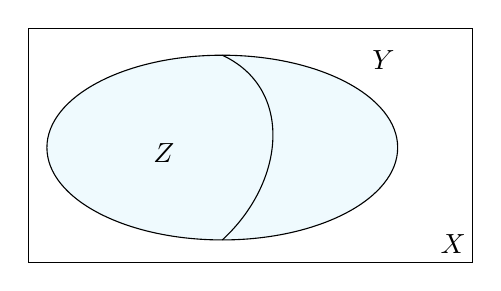
\begin{tikzpicture}[x=0.75pt,y=0.75pt,yscale=-1,xscale=1]
\draw   (100,57) -- (314,57) -- (314,170) -- (100,170) -- cycle ;
\draw  [fill={rgb, 255:red, 239; green, 250; blue, 254 }  ,fill opacity=1 ] (109,114.5) .. controls (109,89.92) and (146.83,70) .. (193.5,70) .. controls (240.17,70) and (278,89.92) .. (278,114.5) .. controls (278,139.08) and (240.17,159) .. (193.5,159) .. controls (146.83,159) and (109,139.08) .. (109,114.5) -- cycle ;
\draw    (193.5,70) .. controls (228,86) and (224,131) .. (193.5,159) ;
\draw (159,111.4) node [anchor=north west][inner sep=0.75pt]    {$Z$};
\draw (264.5,66.4) node [anchor=north west][inner sep=0.75pt]    {$Y$};
\draw (312,166.6) node [anchor=south east] [inner sep=0.75pt]    {$X$};
\end{tikzpicture}
\caption{命题1.4之集合关系图}
\end{figure}
		\item[\lei{[$\supset$]}] 即证$\forall x\in \overline{Z_{X}}\cap Y , \st x\in \overline{Z_{Y}}$,首先明显有$x\in Y$于是仍分类讨论:
		\begin{enumerate}
			\item $x\in Z$显然成立
			\item $x\notin Z$,此时意味着$x$为$Z$在$X$中的极限点,只需证$x\in \overline{Z_{X}}$,即证$x$为$Z$在$Y$中的极限点。
			
			事实上,任意在$Y$中的包含$x$的开集,由子空间拓扑,不妨设之为$V\cap Y$,其中$V\subset_{open} X (x\in V)$,因为$x$为$Z$在$X$中的极限点,所以$(V\chadiao\dkh{x})\cap Z \neq \emptyset$,又由于$x\in Y$,所以$(V\chadiao \dkh{x})\cap Z\cap Y = (V\cap(Y\chadiao\dkh{x}))\cap Z \neq \emptyset$   
		\end{enumerate}
	\end{enumerate}
\end{proof}
更进一步,我们问以下的问题:
\begin{problem}
	设$X$是拓扑空间,$F\subset X$稠密,$U\subset X$,问:$F\cap U$是否在$U$中稠密?
\end{problem}

答案是否定的,因为如果偷鸡取$U = X\chadiao F$这件事就算寄了。于是为了排除这个情况,我们必须要求$U$是开集。如下命题:
\begin{proposition}
		设$X$是拓扑空间,$F\subset X$稠密,$U\subset_{open} X$是$X$且赋予子空间拓扑,则$F\cap U$在$U$中稠密。
\end{proposition}
\begin{proof}
	要证$\overline{(F\cap U)_{U}} = U$根据命题\ref{c1-m4},即要证$\overline{(F\cap U)_{U}}\cap U = U$,即要证$U\subset \overline{(F\cap U)_{X}}$。
	
	即对$\forall x\in U$要证$x\in \overline{(F\cap U)_{X}}$。则分两类讨论:
	\begin{enumerate}
		\item $x\in F\cap U$ 显然成立
		\item $x\notin F\cap U$ ,又由于$F$在$X$中稠密,那么$x$是$F$的极限点,\tl{任取$X$中开集$V(x\in V)$},由于$U$是$X$中开集,因此$V\cap U$也是$X$中开集,因为$x$是$F$的极限点,所以有:
		\begin{equation*}
			\begin{aligned}
				&\xkh{(V\cap U)\chadiao \dkh{x}}\cap F \neq \emptyset\\
				\iff & \tl{(V\chadiao\dkh{x})\cap(F\cap U)\neq \emptyset}
			\end{aligned}
		\end{equation*}
	\end{enumerate}
\end{proof}
\subsection{集合之解体}
为了更好说话,引入以下概念:
\begin{definition}[内点,外点,边界点]
设X为一个拓扑空间,$A\subset X$定义:
\begin{itemize}
	\item 定义$A$的\gn{内点集}:$int(A) : = \dkh{p\in A | \exists X\text{中开集}V(p\in V) , V\subset A}$
	\item 定义$A$的\gn{外点集}:$ext(A) : = \dkh{p\notin A | \exists X\text{中开集}V(p\in V) , V\subset X\chadiao A} \iff int(X\chadiao A)$ 
	\item 定义$A$的\gn{边界点集}:$\partial(A) := \dkh{p\in X | \forall p\text{的开邻域}V,V\cap A \neq \emptyset.V\cap(X\chadiao A) \neq \emptyset}$
\end{itemize}
\end{definition}
\begin{note}
根据以上定义,我们显然有:
\begin{equation*}
	X = int(A) \sqcup ext(A) \sqcup \partial(A)
\end{equation*}
\end{note}
\begin{example}[一些显然的例子]
	\begin{enumerate}
		\item 设$A = [0,1)\subset \mathbb{R}$那么:$\partial(A) = \dkh{0,1} , int(A) = \xkh{0,1} , ext(A) = (-\infty,0)\cup(1,+\infty)$
		\item \begin{enumerate}
		\item 设$A = (0,1)\subset [0,1)$那么:$\partial(A) = \dkh{0} , int(A) = \xkh{0,1} , ext(A) = \emptyset$
		\item 设$A = (0,1)\subset \mathbb{R}$那么:$\partial(A) = \dkh{0,1} , int(A) = \xkh{0,1} , ext(A) = (-\infty,0)\cup(1,+\infty)$
		\end{enumerate}
		\item 设$D = \dkh{(x,y)\in \mathbb{R}^{2}|x^{2}+y^{2}<1} $于是:\begin{enumerate}
		\item $\partial(D) = S^{1} =  \dkh{(x,y)\in \mathbb{R}^{2}|x^{2}+y^{2}=1}$
		\item $int(D) = D$
		\item $ext(D) =  \dkh{(x,y)\in \mathbb{R}^{2}|x^{2}+y^{2}>1}$
		\begin{figure}[h]
			\centering
\tikzset{every picture/.style={line width=0.75pt}}
\begin{tikzpicture}[x=0.75pt,y=0.75pt,yscale=-1,xscale=1]
\draw    (163,135) -- (320,135) ;
\draw [shift={(322,135)}, rotate = 180] [color={rgb, 255:red, 0; green, 0; blue, 0 }  ][line width=0.75]    (10.93,-3.29) .. controls (6.95,-1.4) and (3.31,-0.3) .. (0,0) .. controls (3.31,0.3) and (6.95,1.4) .. (10.93,3.29)   ;
\draw    (238.5,206) -- (238.5,51) ;
\draw [shift={(238.5,49)}, rotate = 90] [color={rgb, 255:red, 0; green, 0; blue, 0 }  ][line width=0.75]    (10.93,-3.29) .. controls (6.95,-1.4) and (3.31,-0.3) .. (0,0) .. controls (3.31,0.3) and (6.95,1.4) .. (10.93,3.29)   ;
\draw  [dash pattern={on 4.5pt off 4.5pt}] (194.25,135) .. controls (194.25,110.56) and (214.06,90.75) .. (238.5,90.75) .. controls (262.94,90.75) and (282.75,110.56) .. (282.75,135) .. controls (282.75,159.44) and (262.94,179.25) .. (238.5,179.25) .. controls (214.06,179.25) and (194.25,159.44) .. (194.25,135) -- cycle ;
\draw (324,138.4) node [anchor=north west][inner sep=0.75pt]    {$x$};
\draw (240.5,52.4) node [anchor=north west][inner sep=0.75pt]    {$y$};
\draw (284.75,138.4) node [anchor=north west][inner sep=0.75pt]    {$1$};
\draw (240.5,138.4) node [anchor=north west][inner sep=0.75pt]    {$0$};
\end{tikzpicture}
\caption{例1.18.3之拓扑空间$D$}
		\end{figure}
		\end{enumerate}
		\item 设$A = [0,1]\subset \mathbb{R}^{2}$,此时$\partial(A) = A , int(A) = \emptyset , ext(A) = X\chadiao A$
		\begin{figure}[h]
			\centering
\tikzset{every picture/.style={line width=0.75pt}}
\begin{tikzpicture}[x=0.75pt,y=0.75pt,yscale=-1,xscale=1]
\draw    (100,128) -- (261,128) ;
\draw [shift={(263,128)}, rotate = 180] [color={rgb, 255:red, 0; green, 0; blue, 0 }  ][line width=0.75]    (10.93,-3.29) .. controls (6.95,-1.4) and (3.31,-0.3) .. (0,0) .. controls (3.31,0.3) and (6.95,1.4) .. (10.93,3.29)   ;
\draw    (140,172) -- (140,86) ;
\draw [shift={(140,84)}, rotate = 90] [color={rgb, 255:red, 0; green, 0; blue, 0 }  ][line width=0.75]    (10.93,-3.29) .. controls (6.95,-1.4) and (3.31,-0.3) .. (0,0) .. controls (3.31,0.3) and (6.95,1.4) .. (10.93,3.29)   ;
\draw [color={rgb, 255:red, 208; green, 2; blue, 27 }  ,draw opacity=1 ]   (140,128) -- (176,128) ;\draw (142,131.4) node [anchor=north west][inner sep=0.75pt]    {$0$};
\draw (178,131.4) node [anchor=north west][inner sep=0.75pt]    {$1$};
\draw (265,131.4) node [anchor=north west][inner sep=0.75pt]    {$x$};
\draw (142,87.4) node [anchor=north west][inner sep=0.75pt]    {$y$};
\end{tikzpicture}
\caption{例1.18.4之拓扑空间$A$}
		\end{figure}
	\end{enumerate}
\end{example}
\section{拓扑空间的砖头---拓扑基}
\begin{definition}[拓扑基]
	设$X$是拓扑空间,$\tpj$是一个由一些$X$中开集构成的集族,如果对$\forall X$中开集$U$,$U$均可表为$\tpj$中一些元素之并,则称$\tpj$构成了$X$的一个\gn{拓扑基}。
\end{definition}
\begin{example}[$\mathbb{R}^{1}$中的欧氏拓扑可以有不同的拓扑基]
\label{c1-e19}
	很明显,$\mathbb{R}^{1}$有一个拓扑基为$\tpj = \dkh{(a,b)|a<b}$。
	
	令$\tpj '  = \dkh{(a,b)|a<b,a,b\in \mathbb{Q}}$,则$\tpj ' $也是$\mathbb{R}^{1}$的一个拓扑基。
	\begin{proof}
		$\forall U\subset_{open} \mathbb{R}^{1},\forall p\in U$,则存在$a<p<b$使得$(a,b)\subset U$,从而由有理数集的稠密性可知,$\exists(a_{p},b_{p})\in \tpj',\st p\in (a_{p},b_{p})\subset U$即$U = \dajiao_{p\in U}(a_{p},b_{p})$。
		\begin{figure}[h]
			\centering
\tikzset{every picture/.style={line width=0.75pt}}
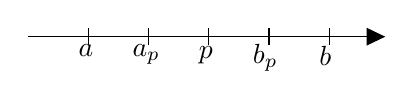
\begin{tikzpicture}[x=0.75pt,y=0.75pt,yscale=-1,xscale=1]
\draw    (100,101) -- (212,101) -- (227,101) -- (269,101) (129,97) -- (129,105)(158,97) -- (158,105)(187,97) -- (187,105)(216,97) -- (216,105)(245,97) -- (245,105) ;
\draw [shift={(272,101)}, rotate = 180] [fill={rgb, 255:red, 0; green, 0; blue, 0 }  ][line width=0.08]  [draw opacity=0] (8.93,-4.29) -- (0,0) -- (8.93,4.29) -- cycle    ;
\draw (181,104.4) node [anchor=north west][inner sep=0.75pt]    {$p$};
\draw (123,103.4) node [anchor=north west][inner sep=0.75pt]    {$a$};
\draw (239,104.4) node [anchor=north west][inner sep=0.75pt]    {$b$};
\draw (149,103.4) node [anchor=north west][inner sep=0.75pt]    {$a_{p}$};
\draw (207,103.4) node [anchor=north west][inner sep=0.75pt]    {$b_{p}$};
\end{tikzpicture}
\caption{例1.19之数轴}
		\end{figure}
	\end{proof}
\end{example}
\begin{note}
由此可见,一个拓扑空间可以有诸多拓扑基,但是一个拓扑基是否唯一确定一个拓扑空间呢?答案是肯定的,这个结论将由以下讨论给出。	
\end{note}

了解了定义,我们就需要探究一个拓扑基$\tpj$之所以为拓扑基的等价条件。很明显,由拓扑基我们可以知道拓扑基的必要条件,如下面这个命题:
\begin{proposition}
	设$X$为拓扑空间,$\tpj$为$X$的一个拓扑基,那么:
	\begin{enumerate}
		\item[\lei{TB1}]. $\dabing_{U\in \tpj}U = X$
		\item[\lei{TB2}]. $\forall U_{1},U_{2}\in \tpj \st U_{1}\cap U_{2}$可以表示为$\tpj$中一些元素之并。
	\end{enumerate}
\end{proposition}

\begin{proof}
	显然。
\end{proof}

这个命题反过来也是正确的,即有以下的命题:
\begin{proposition}
	设$X$为一个集合,$\tpj$为$X$的一个由一些子集构成的集族,若$\tpj$满足以上\lei{TB1}、\lei{TB2}两条,则$\tpj$必为$X$上某个拓扑$\tp$的拓扑基。而且,$\tp$是唯一的,称之为由拓扑基$\tpj$\gn{生成}的拓扑。
\end{proposition}
\begin{proof}
	定义$\tp=\dkh{\emptyset}\cup\dkh{\tpj\text{中若干元素之并}}=\dkh{\bigcup_{\alpha\in I}U_{\alpha}|U_{\alpha}\in \tpj}\cup\dkh{\emptyset}$,我们所要证明的是以下两点:
	\begin{enumerate}
		\item $\tp$是$X$上的一个拓扑。
	事实上,我们有:
	\begin{enumerate}
		\item $\emptyset , X\in \tp$(显然,由定义和条件\lei{TB1}可以保证。)
		\item $\tp$对于任意并封闭是显然的(因为就是这样定义的。)
		\item 对于$\forall \dabing_{\alpha \in I}U_{\alpha} , \dabing_{\beta\in J}V_{\beta}\in \tp$,其中$U_{\alpha},V_{\beta}\in \tpj,\forall \alpha \in I,\beta\in J$那么有:
		\begin{equation*}
			\xkh{\dabing_{\alpha\in I}U_{\alpha}}\cap\xkh{\dabing_{\beta\in J}V_{\beta}} = \dajiao_{\alpha,\beta}(U_{\alpha}\cap V_{\beta}) \in \tp
		\end{equation*}
	\end{enumerate}
	\item $\tpj$为拓扑$\tp$上的一个拓扑基。
	\end{enumerate}
	根据定义可知$\tpj$也确实为拓扑$\tp$上的一个拓扑基。从构造来看,我们并没有规定在拓扑基$\tpj$中的并是哪些,因此$\tp$是唯一的,因此命题得证。
\end{proof}
\begin{example}[$\mathbb{R}^{2}$的另一拓扑基]
	明显来看,欧氏空间$\mathbb{R}^{2}$中的开球的全体构成的集合是$\mathbb{R}^{2}$的一个拓扑基,根据我们在度量空间中所积攒的经验,$\mathbb{R}^{2}$中的开球和邻域是等价的,很自然的我们可以考虑$\mathbb{R}^{2}$中的开矩体的全体构成的集合$\tpj' = \dkh{(a,b)\times(c,d)|a<b,c<d}\cup\dkh{\emptyset}$:
	\begin{figure}[h]
		\centering
\tikzset{every picture/.style={line width=0.75pt}}
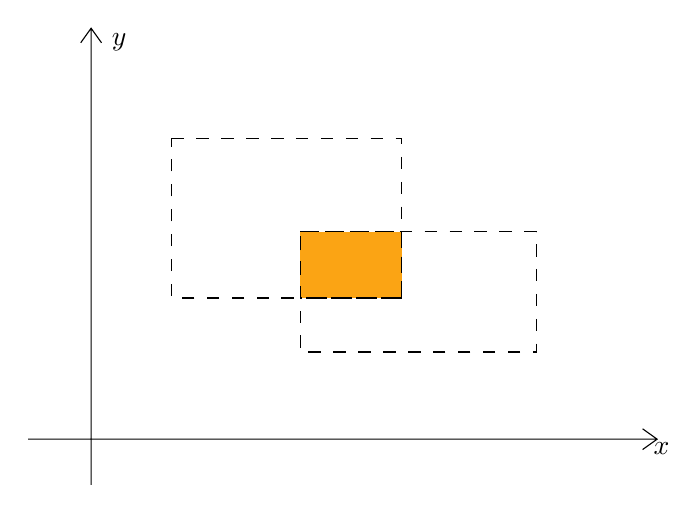
\begin{tikzpicture}[x=0.75pt,y=0.75pt,yscale=-1,xscale=1]
\draw  (43,229) -- (346,229)(73.3,31) -- (73.3,251) (339,224) -- (346,229) -- (339,234) (68.3,38) -- (73.3,31) -- (78.3,38)  ;
\draw  [fill={rgb, 255:red, 251; green, 164; blue, 20 }  ,fill opacity=1 ][dash pattern={on 4.5pt off 4.5pt}] (223,161) -- (174,161) -- (174,129) -- (223,129) -- (223,161) -- cycle ;
\draw  [dash pattern={on 4.5pt off 4.5pt}] (112,84) -- (223,84) -- (223,161) -- (112,161) -- cycle ;
\draw  [dash pattern={on 4.5pt off 4.5pt}] (174,129) -- (288,129) -- (288,187) -- (174,187) -- cycle ;
\draw (343,229.4) node [anchor=north west][inner sep=0.75pt]    {$x$};
\draw (82,32.4) node [anchor=north west][inner sep=0.75pt]    {$y$};
\end{tikzpicture}
\caption{例1.20之开矩体}
	\end{figure}
	
	很明显$\tpj'$是$\mathbb{R}^{2}$上某拓扑的拓扑基。
\end{example}
为了更好地描述两个拓扑基之间的关系,以便更加方便地研究两个拓扑基生成的拓扑空间之间的关系,我们对拓扑基引入如下的定义:
\begin{definition}[拓扑基之间的等价]
设$\tpj,\tpj'$满足\lei{TB1}、\lei{TB2},称$\tpj$与$\tpj'$是\gn{等价}的,若:
\begin{enumerate}
	\item $\forall U\in \tpj,p\in U,$都$\exists U'\in \tpj',\st p\in U'\subset U$
	\item $\forall V\in \tpj',p'\in V',$都$\exists V\in \tpj',\st p\in V\subset V'$
\end{enumerate}
\end{definition}

\begin{figure}[h]
\centering
 {
  \begin{minipage}{5cm}
   \centering
\tikzset{every picture/.style={line width=0.75pt}}
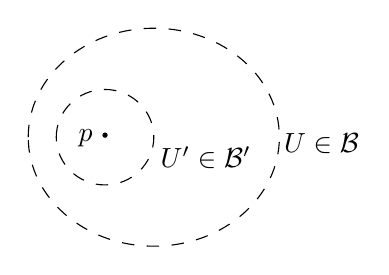
\begin{tikzpicture}[x=0.75pt,y=0.75pt,yscale=-1,xscale=1]
\draw  [dash pattern={on 4.5pt off 4.5pt}] (105,146.5) .. controls (105,117.51) and (132.09,94) .. (165.5,94) .. controls (198.91,94) and (226,117.51) .. (226,146.5) .. controls (226,175.49) and (198.91,199) .. (165.5,199) .. controls (132.09,199) and (105,175.49) .. (105,146.5) -- cycle ;
\draw  [dash pattern={on 4.5pt off 4.5pt}] (118.5,146.5) .. controls (118.5,133.8) and (129.02,123.5) .. (142,123.5) .. controls (154.98,123.5) and (165.5,133.8) .. (165.5,146.5) .. controls (165.5,159.2) and (154.98,169.5) .. (142,169.5) .. controls (129.02,169.5) and (118.5,159.2) .. (118.5,146.5) -- cycle ;
\draw  [fill={rgb, 255:red, 0; green, 0; blue, 0 }  ,fill opacity=1 ] (141,145.5) .. controls (141,144.95) and (141.45,144.5) .. (142,144.5) .. controls (142.55,144.5) and (143,144.95) .. (143,145.5) .. controls (143,146.05) and (142.55,146.5) .. (142,146.5) .. controls (141.45,146.5) and (141,146.05) .. (141,145.5) -- cycle ;
\draw (128,141.4) node [anchor=north west][inner sep=0.75pt]    {$p$};
\draw (167.5,149.9) node [anchor=north west][inner sep=0.75pt]    {$U'\in \tpj'$};
\draw (227,143.4) node [anchor=north west][inner sep=0.75pt]    {$U\in \tpj$};
\end{tikzpicture}
  \end{minipage}
 }
    {
     \begin{minipage}{6cm}
      \centering
      \tikzset{every picture/.style={line width=0.75pt}}
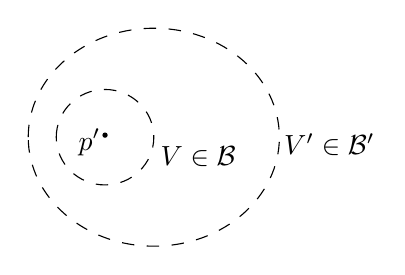
\begin{tikzpicture}[x=0.75pt,y=0.75pt,yscale=-1,xscale=1]
\draw  [dash pattern={on 4.5pt off 4.5pt}] (105,146.5) .. controls (105,117.51) and (132.09,94) .. (165.5,94) .. controls (198.91,94) and (226,117.51) .. (226,146.5) .. controls (226,175.49) and (198.91,199) .. (165.5,199) .. controls (132.09,199) and (105,175.49) .. (105,146.5) -- cycle ;
\draw  [dash pattern={on 4.5pt off 4.5pt}] (118.5,146.5) .. controls (118.5,133.8) and (129.02,123.5) .. (142,123.5) .. controls (154.98,123.5) and (165.5,133.8) .. (165.5,146.5) .. controls (165.5,159.2) and (154.98,169.5) .. (142,169.5) .. controls (129.02,169.5) and (118.5,159.2) .. (118.5,146.5) -- cycle ;
\draw  [fill={rgb, 255:red, 0; green, 0; blue, 0 }  ,fill opacity=1 ] (141,145.5) .. controls (141,144.95) and (141.45,144.5) .. (142,144.5) .. controls (142.55,144.5) and (143,144.95) .. (143,145.5) .. controls (143,146.05) and (142.55,146.5) .. (142,146.5) .. controls (141.45,146.5) and (141,146.05) .. (141,145.5) -- cycle ;
\draw (128,141.4) node [anchor=north west][inner sep=0.75pt]    {$p'$};
\draw (167.5,149.9) node [anchor=north west][inner sep=0.75pt]    {$V\in \tpj$};
\draw (227,143.4) node [anchor=north west][inner sep=0.75pt]    {$V'\in \tpj'$};
\end{tikzpicture}
     \end{minipage}
    }
		\caption{定义1.10的说明}
	\end{figure}
	
	\begin{proposition}
		设$\tpj$与$\tpj'$满足\lei{TB1}、\lei{TB2},且$\tpj$与$\tpj'$等价,则$\tpj$生成的拓扑$\tp$与$\tpj'$生成的拓扑$\tp'$相同。
	\end{proposition}
	\begin{proof}
		证明很简单,$\forall U\in \tp ~\Rightarrow ~U = \dabing_{\alpha\in I}U_{\alpha},U_{\alpha}\in \tpj$,又因为两个拓扑基等价,则有:
		
		$$\forall U_{\alpha},\forall p\in U_{\alpha} ~\Rightarrow ~\exists V_{p}\in \tpj',\st p\in V_{p}\subset U_{\alpha}$$
		
		即:$U_{\alpha} = \dabing_{p\in U_{\alpha}}V_{p}\in \tp'$,即$U = \dabing_{\alpha \in I}U_{\alpha}\in \tp'$,则$\tp\subset\tp'$
		
		同理,$\tp\subset\tp'$,因此$\tp=\tp'$
	\end{proof}
	
	为了更好的使用以上拓扑基的等价条件,我们可以篡改\lei{TP2}为以下的\lei{TP2'}:
	\begin{enumerate}
		\item[\lei{TP2'}]. $\forall U_{1},U_{2}\in \tpj , \forall p\in U_{1}\cap U_{2},\exists U_{p}\in \tpj, \st p\in U_{p}\subset U_{1}\cap U_{2}$
	\end{enumerate}
	\begin{proof}
		这个的验证也十分显然。
	\end{proof}
%第二章
\chapter{连续映射}
研究点集拓扑的主要动机就是从更加一般的观点来定义连续性、紧性和连通性。下面三章就是在做这个工作。这一章,先研究一般的连续映射\footnote{值得强调的是,在尤承业老师的《基础拓扑学》中36页提到,除此之外还有\textbf{可数性}、\textbf{分离性},这些也贯穿在这几章中出现。} 。
\section{连续映射}
首先,我们重申连续性的定义:

\begin{definition}[连续映射]
	若$f$是拓扑空间$X\longrightarrow Y$的映射,如果$\forall ~U\subset_{open} Y , f^{-1}(U)$为$X$中开集,则称映射$f$是\gn{连续映射}。
\end{definition}
我们有下面这俩显然的命题:\begin{proposition}[连续映射之复合是连续映射]
	设$X,Y,Z$是三个拓扑空间,定义连续映射$f:X\longrightarrow Y$,$g:X\longrightarrow Y$,则$gf:X\longrightarrow Z$是连续映射。
\end{proposition}
\begin{proof}
	对于$\forall U\subset_{open} Z$,我们有$(g \cdot f)^{-1}(U) =f^{-1} (g^{-1}(U))$,由于$g$是连续映射,则$g^{-1}(U)$是$Y$中的开集;又由$f$是连续映射,所以$f^{-1} (g^{-1}(U))$是$X$中开集。
\end{proof}

\begin{proposition}[连续映射之限制是连续映射]
	设$f:X\longrightarrow Y$是连续映射,$A\subset X$并赋予$A$以子空间拓扑,那么$f|_{A}:A\longrightarrow Y$是连续映射。
\end{proposition}
\begin{proof}
	$\forall U\subset_{open} Y, $因为赋予$A$以子空间拓扑,所以有$(f|_{A})^{-1}(U) = A\cap f^{-1}(U)$
	
	又由于$f$是$X\longrightarrow Y$的连续映射,所以$f^{-1}(U)$是$X$中开集,所以$A\cap f^{-1}(U)$就为$A$中开集。
\end{proof}

\section{充满整个空间的曲线-Peano\footnote{朱塞佩·皮亚诺 (意大利语:Giuseppe Peano;1858年8月27日-1932年4月20日)是意大利数学家、逻辑学家、语言学家。}曲线}
%第三章
\chapter{紧性}
%第四章
\chapter{连通性}
%符号说明
\chapter{符号说明}
%\begin{mdframed}
%	一切没有符号说明的文档都是耍流氓!
%	
%	\hfill---my帅气的作者\quad
%\end{mdframed}

本讲义有以下符号说明,便于我自己看不明白的时候过来回顾一下(
\section{符号说明}
\begin{enumerate}
	\item $O\subset_{open}X$的含义是$O$是$X$的开子集。
	\item $F\subset_{closed}X$的含义是$F$是$X$的闭子集。
	\item $F=_{closed}X$的含义是$F$和$X$相等,且均为闭集。
	\item 所有的弯体(比如$\subset$)变直之后就表示更加强的区分效果(比如$\sqsubset$,表示真被包含)。
	\item 所有的包含采用类似$\subset$的符号,若出现$\subseteq$(一般不会),表示同一意思。
\end{enumerate}
\section{语法说明}
\begin{enumerate}
	\item 数学逻辑语言同国际标准。
	\item 外加一些张氏古代汉语和标准中式英语(虽然掺杂一些少量标准英式英语)。
\end{enumerate}
\end{document}
